\documentclass[final,hyperref={pdfpagelabels=false}]{beamer}

\mode<presentation>{\usetheme{I6pd2_hugo}}
\usepackage[english]{babel}
\usepackage[utf8]{inputenc}
\usepackage{amsmath,amsthm, amssymb, latexsym, subfigure, graphicx,array,booktabs,tabularx, caption}
%\usepackage{times}\usefonttheme{professionalfonts}  % obsolete
%\usefonttheme[onlymath]{serif}
\boldmath
\usepackage[orientation=portrait,size=a0,scale=1.4,debug]{beamerposter}
% change list indention level
% \setdefaultleftmargin{3em}{}{}{}{}{}
\usecaptiontemplate{
\small
\structure{\insertcaptionname~\insertcaptionnumber:}
\insertcaption
}


%\usepackage{snapshot} % will write a .dep file with all dependencies, allows for easy bundling

\newcolumntype{Z}{>{\centering\arraybackslash}X} % centered tabularx columns
\newcommand{\pphantom}{\textcolor{ta3aluminium}} % phantom introduces a vertical space in p formatted table columns??!!

\listfiles

%%%%%%%%%%%%%%%%%%%%%%%%%%%%%%%%%%%%%%%%%%%%%%%%%%%%%%%%%%%%%%%%%%%%%%%%%%%%%%%%%%%%%%

\title{Impedance Studies of the LHC Injection Kicker Magnets for HL-LHC}
\author{H. Day, M.J. Barnes, L. Feliciano}
\institute[CERN]{CERN, Geneva, Switzerland}
\date[June 2014]{June 2014}

%%%%%%%%%%%%%%%%%%%%%%%%%%%%%%%%%%%%%%%%%%%%%%%%%%%%%%%%%%%%%%%%%%%%%%%%%%%%%%%%%%%%%%
\newlength{\columnheight}
\setlength{\columnheight}{105cm}


%%%%%%%%%%%%%%%%%%%%%%%%%%%%%%%%%%%%%%%%%%%%%%%%%%%%%%%%%%%%%%%%%%%%%%%%%%%%%%%%%%%%%%
\begin{document}
\begin{frame}
  \begin{columns}
    % ---------------------------------------------------------%
    % Set up a column 
    \begin{column}{.49\textwidth}
      \begin{beamercolorbox}[center,wd=\textwidth]{postercolumn}
        \begin{minipage}[T]{.95\textwidth}  % tweaks the width, makes a new \textwidth
          \parbox[t][\columnheight]{\textwidth}{ % must be some better way to set the the height, width and textwidth simultaneously
            % Since all columns are the same length, it is all nice and tidy.  You have to get the height empirically
            % ---------------------------------------------------------%
            % fill each column with content            
            \begin{block}{Summary}
\small{
The LHC injection kicker magnets (MKIs) experienced strong heating during the first operational run, identified as being caused by power loss due to wakefields induced by circulating beam. Studies of the beam coupling impedance of the beam screen, a series of conductors embedded in a ceramic tube placed in the aperture of the ferrite yoke to screen the ferrite from the beam, resulted in new design offering improved screening: this is predicted to reduce the heating to acceptable levels for operation with 25ns beam during run 2 of the LHC. However higher beam intensities proposed for HL-LHC operation are predicted to again cause strong heating to occur. Further studies have been carried out to reduce the beam induced power loss by optimising the beam screen design, some key results and findings of which are presented here.
}
\end{block}
            \vfill
	\begin{block}{Background}
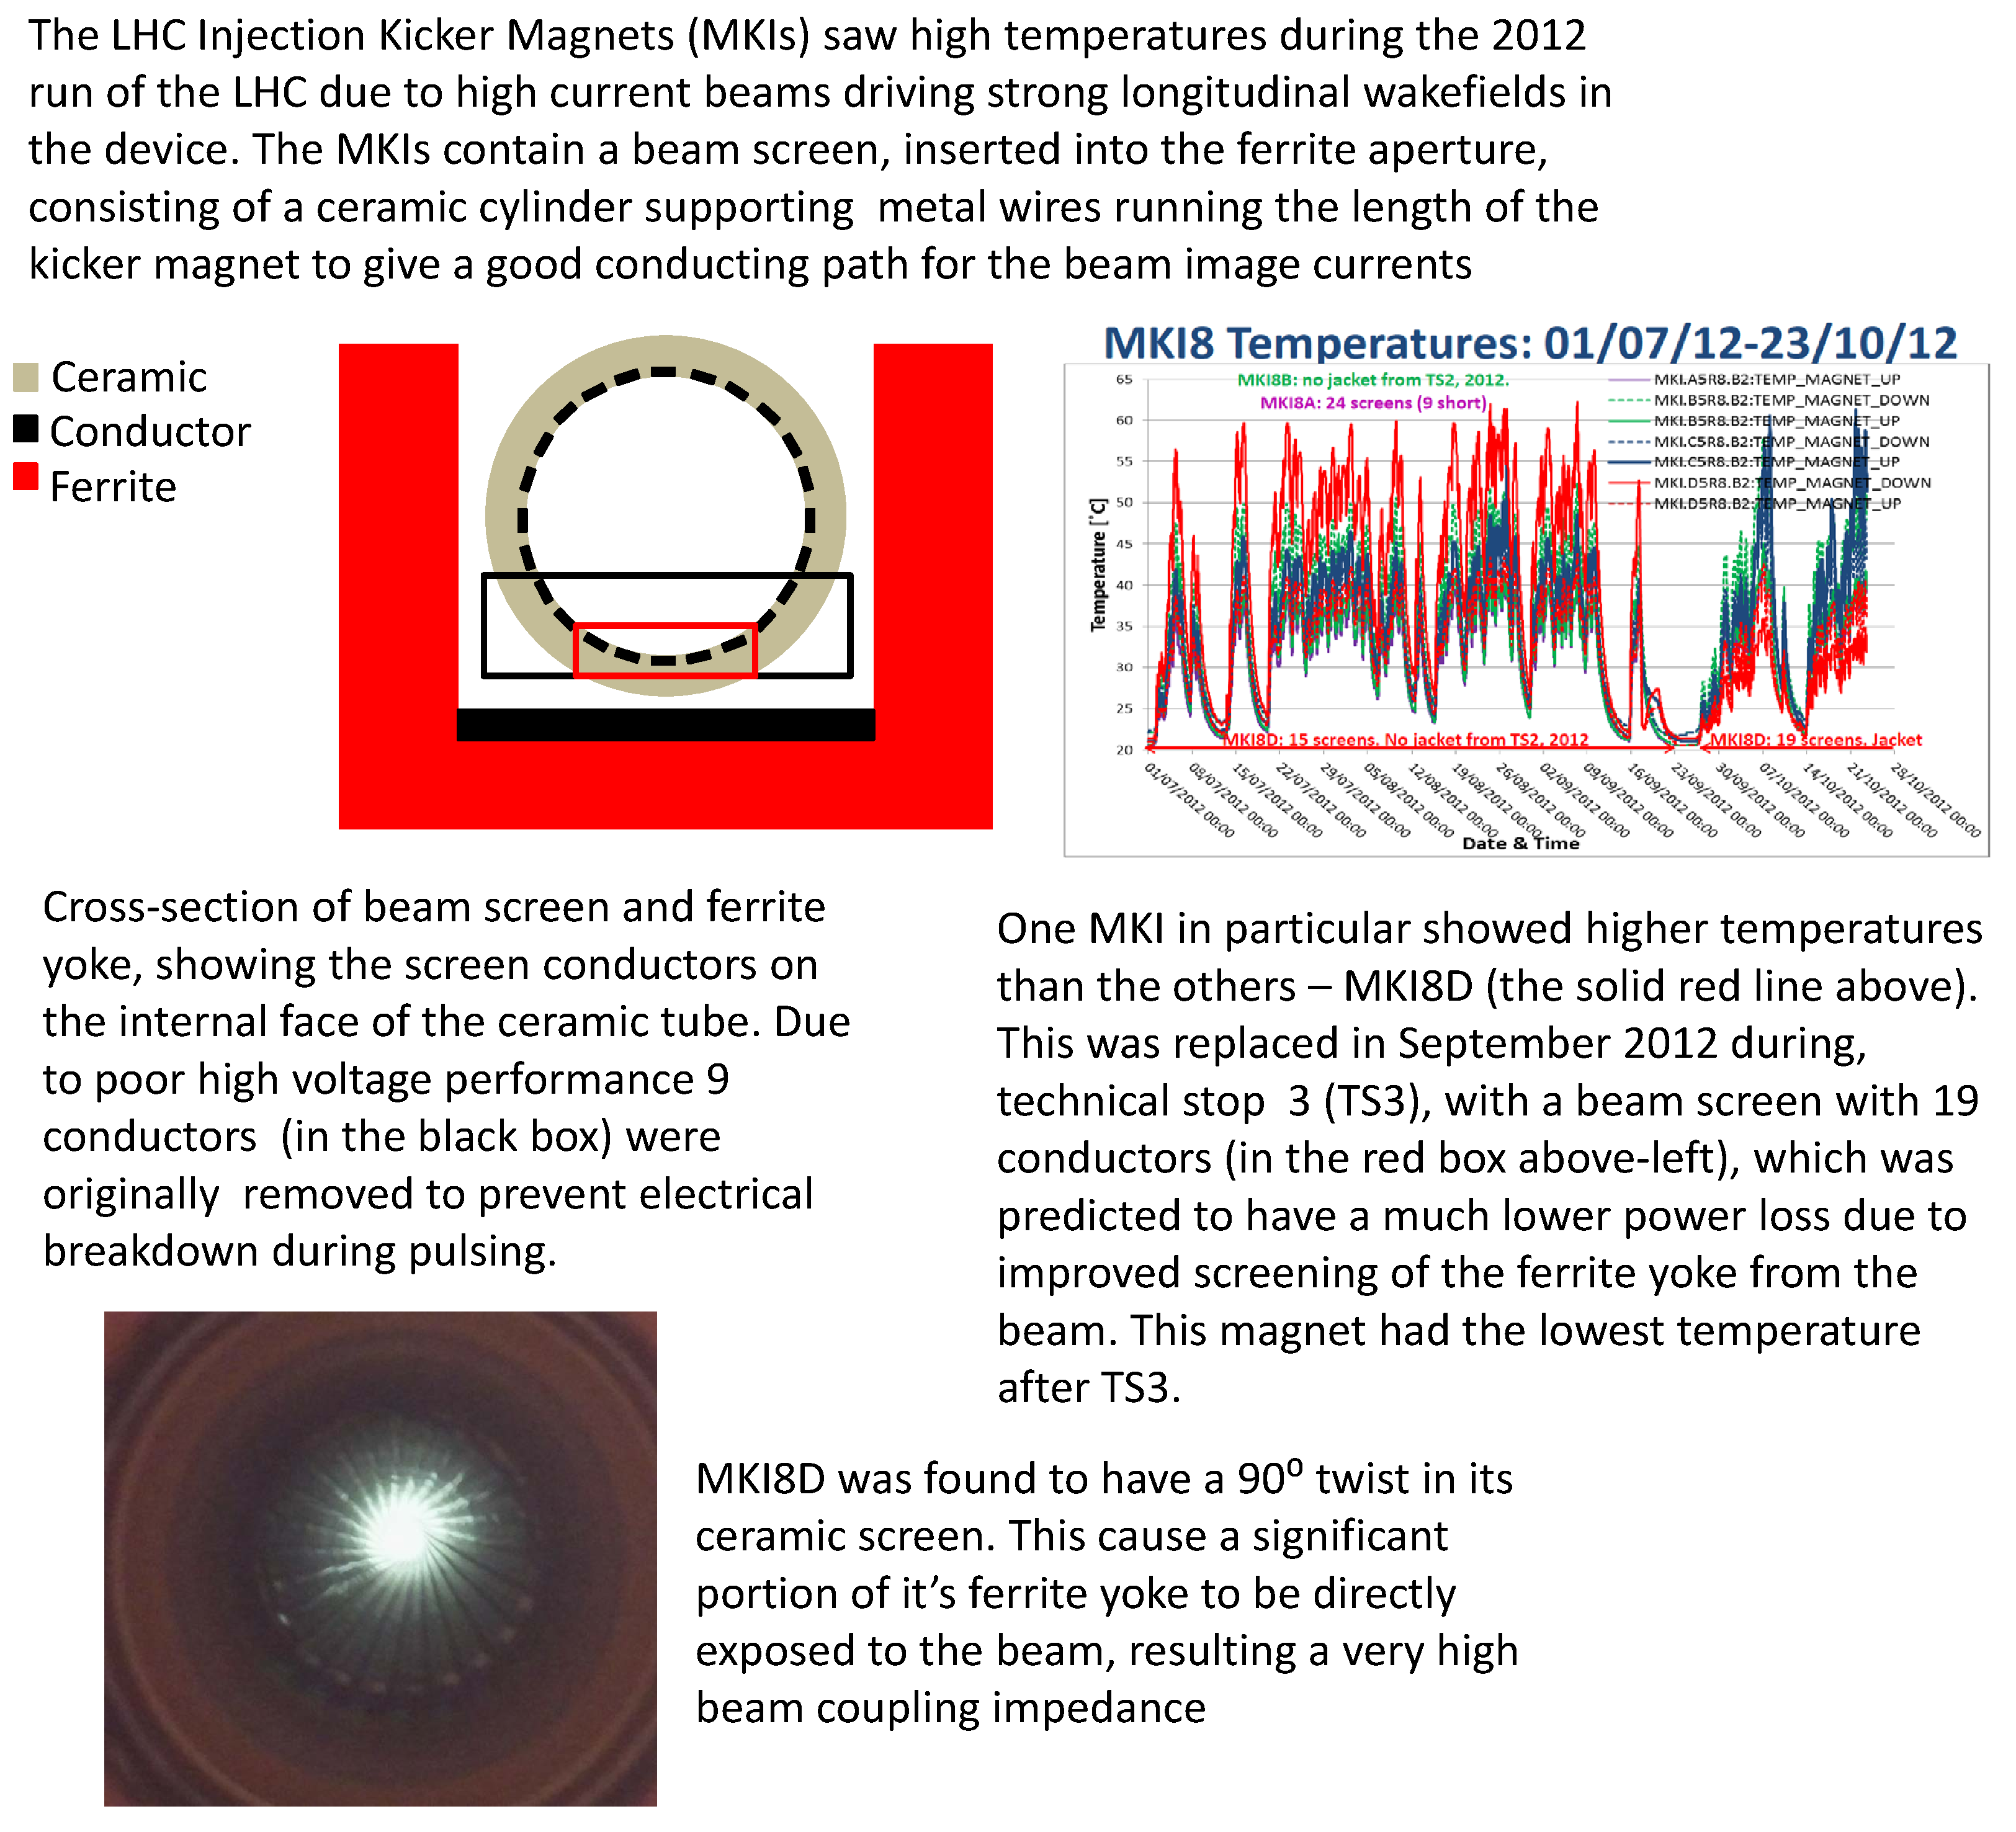
\includegraphics[width=1.0\textwidth]{introductionPicture.pdf}
	\end{block}
 \vfill
	\begin{block}{Beam Screen}
\begin{figure}
\subfigure[]{
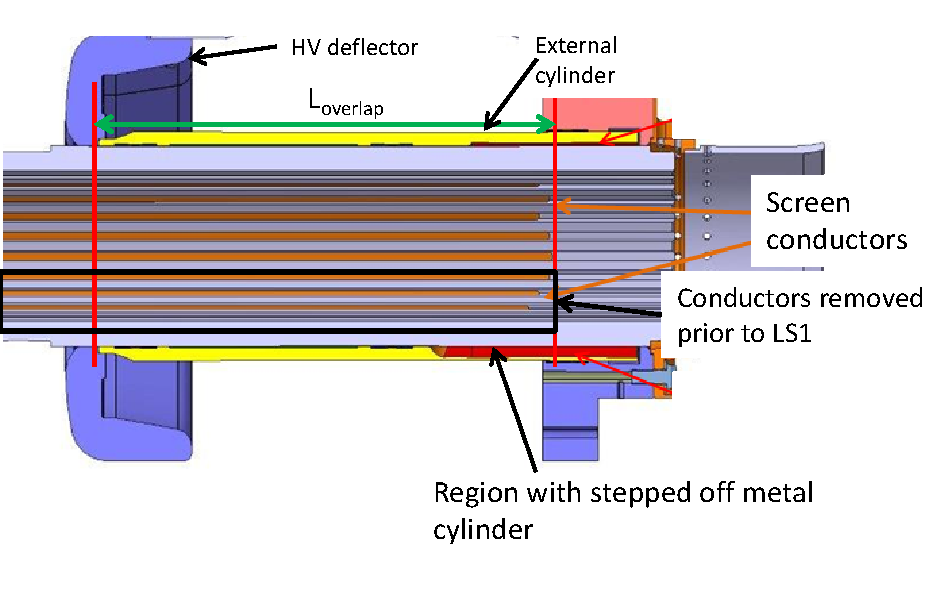
\includegraphics[width=0.55\textwidth]{beamScreenCrossSectionLabelled.pdf}
}\subfigure[]{
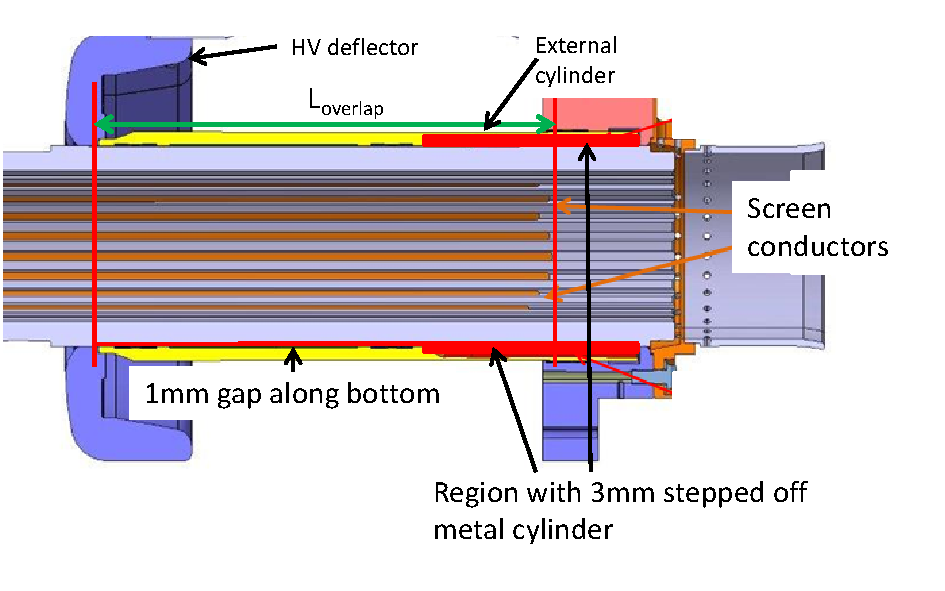
\includegraphics[width=0.55\textwidth]{HLLHCLayout.pdf}
}\end{figure}

\begin{itemize}
\item{The new screen design [1], being installed  in the MKIs during long shutdown 1 (LS1), has been designed to permit the inclusion of 24 screen conductors in the ceramic tube, whilst lowering the surface electric field on the ceramic tube during kicker pulsing to reduce the change of surface flashover.}
\item{The capacitively coupled end is significantly changed:}
\begin{itemize}
\item{The external metallization is replaced by an external metal tube which steps away from the ceramic tube near the ends of the screen conductors. This reduces the surface electric field on the ceramic tube significantly. Tapering the length of the conductors also helps this reduction.}
\item{This allows 24 screen conductors to be placed back in the beam screen, greatly improving the screening of the ferrite yoke from the beam.}
\end{itemize}
\end{itemize}

	\end{block}

            \vfill

\vfill
\begin{block}{References}
\begin{enumerate}
\item{\small{M.J. Barnes \emph{et al}., \emph{Upgrade of the LHC Injection Kicker Magnets}, IPAC2013, MOPWA030}}
\item{\small{M.J. Barnes \emph{et al}., \emph{Cooling of the LHC Injection Kicker Magnet Ferrite Yoke: Measurements and Future Proposals}, MOPME075, These proceedings}}
\item{\small{Hugo Day, PhD Thesis, June 2013}}
\end{enumerate}
\end{block}
         \vfill
          }
        \end{minipage}
      \end{beamercolorbox}
    \end{column}
    % ---------------------------------------------------------%
    % end the column

    % ---------------------------------------------------------%
    % Set up a column 
    \begin{column}{.49\textwidth}
      \begin{beamercolorbox}[center,wd=\textwidth]{postercolumn}
        \begin{minipage}[T]{.95\textwidth} % tweaks the width, makes a new \textwidth
          \parbox[t][\columnheight]{\textwidth}{ % must be some better way to set the the height, width and textwidth simultaneously
            % Since all columns are the same length, it is all nice and tidy.  You have to get the height empirically
            % ---------------------------------------------------------%
            % fill each column with content
\begin{block}{Impedance Measurements of New Design}
\begin{itemize}
\begin{small}
\item{The beam coupling impedance for all MKIs with the new beam screen design is measured before bake out and HV conditioning to ensure consistency between magnets and to foresee any possible problems with regards to heating.}
\item{Measurements are typically done using the coaxial resonant method due to it's sensivity to low impedances.}
\end{small}
\end{itemize}
\begin{figure}
\subfigure[]{
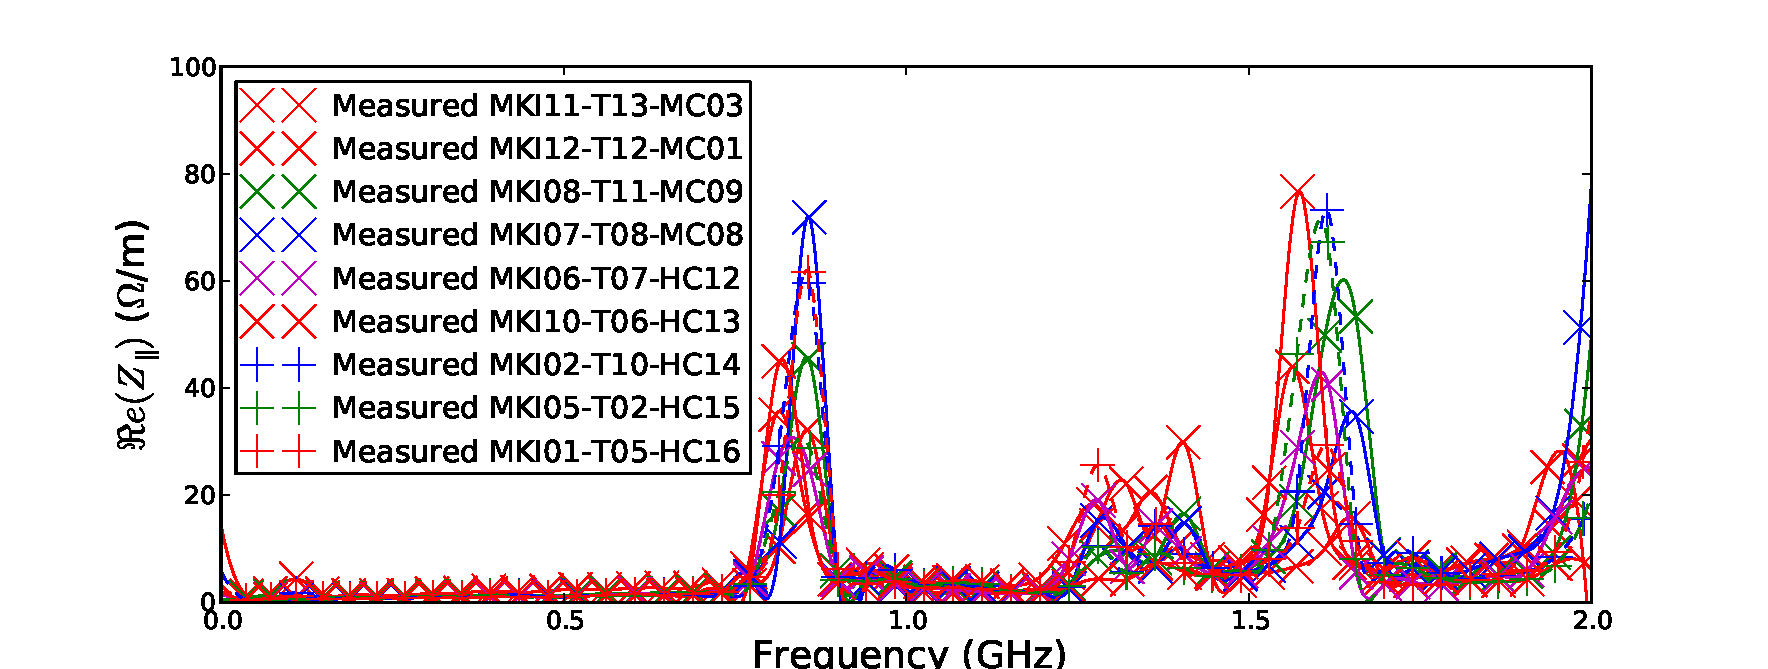
\includegraphics[width=0.45\textwidth]{TUPRI030f4.pdf}
\label{fig:allMKIsNew}
}
\subfigure[]{
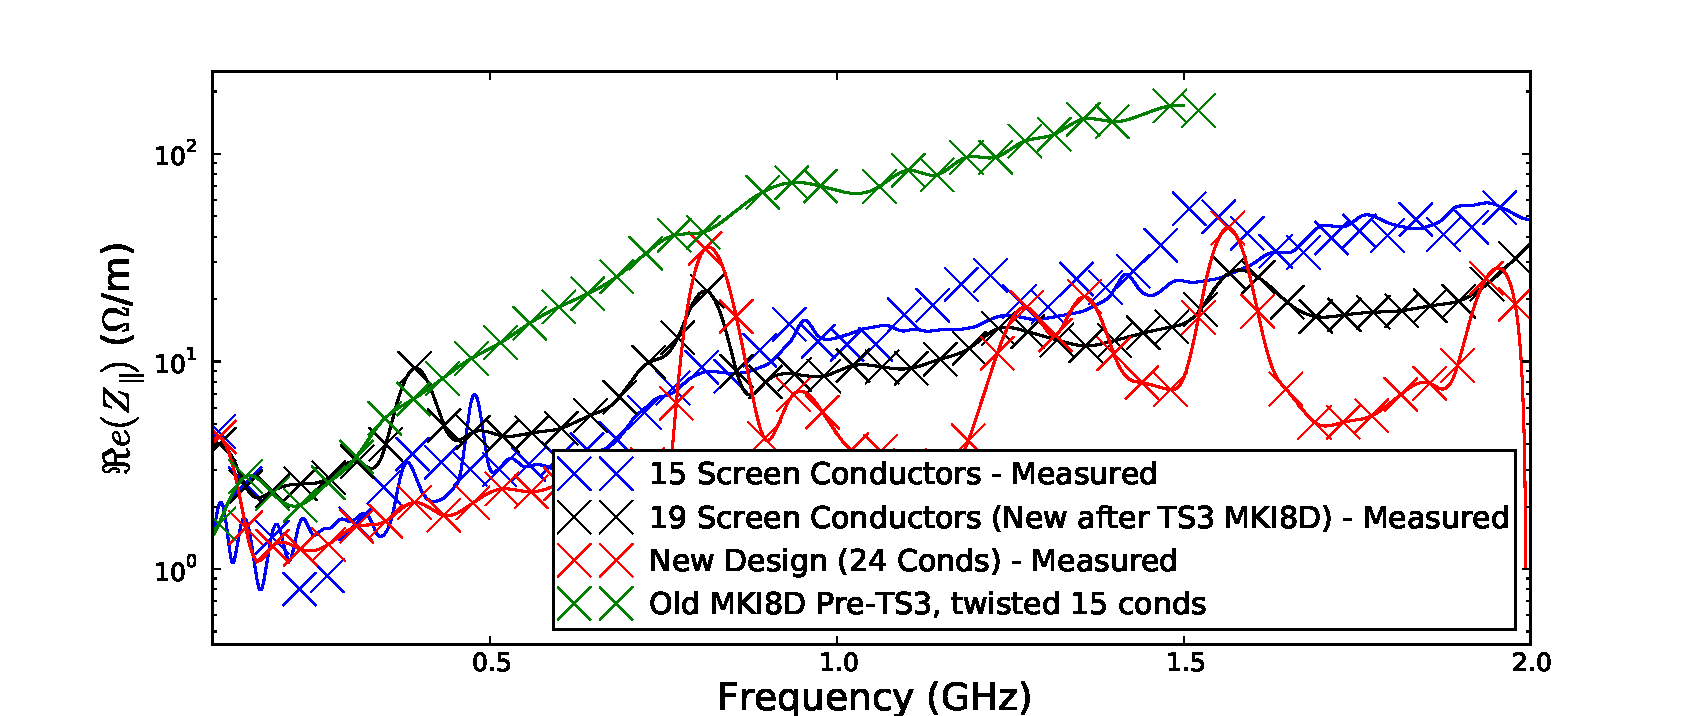
\includegraphics[width=0.45\textwidth]{TUPRI030f3.pdf}
\label{fig:MKIsCondsNumber}
}\caption*{\small{Impedance measurements of \subref{fig:allMKIsNew} all MKIs with the new design using the resonant coaxial wire method and  \subref{fig:MKIsCondsNumber} MKIs with 15, 19 and 24 screen conductors, and the MKI8D pre TS3 (experienced high temperatures)}}
\end{figure}
\begin{table}
\label{tab:beamPar}
\caption*{Beam parameters for power loss calculations}
\begin{center}
\begin{tabular}{c | c | c | c | c}
\small{Running Mode} & $N_{b}$ $10^{11}$ & $n_{bunches}$ & bunch length (ns) & Bunch separation (ns) \\ \hline 
\small{Pre-LS1} & 1.6 & 1380 & 1.2 & 50 \\ \hline
\small{Post-LS1} & 1.15 & 2808 & 1.0 & 25 \\ \hline
\small{HL-LHC 25ns}& 2.2 & 1380 & 1.0 & 25 \\ \hline
\small{HL-LHC 50ns}& 3.5 & 2808 & 1.0 & 50 \\
\end{tabular}
\end{center}
\end{table}

\begin{table}
\label{tab:heating-mki-screen-designs}
\caption*{\small{The power loss expected  in the MKIs for the magnets measured so far. All power losses are given in W/m.}}
\begin{center}
\begin{tabular}{c | c | c | c | c}
\small{Screen Design} & \small{Pre-LS1} & \small{Post-LS1} & \small{HL-LHC 50ns} & \small{HL-LHC 25ns} \\ \hline 
\small{New Design (24 conductors)} & 20-35 & 34-52 & 151-240 & 125-191 \\ \hline
\small{15 screen conductors} & 68 & 117 & 538 & 432 \\ \hline
\small{Old MKI8D (twisted, 15 conds)} & 168 & N/A & N/A & N/A \\ \hline
\small{19 screen conductors} & 52 & 76 & N/A & N/A \\
\end{tabular}
\end{center}
\end{table}
\begin{itemize}
\item{The new design with 24 conductors gives a decrease of some 20-50\% for post-LS1 parameters compared to the magnets with 15 screen conductors pre-LS1 - a great success! It is predicted that beam-induced heating should no longer be a problem in the MKIs for nominal LHC parameters.}
\end{itemize}

\end{block}
\vfill
\begin{block}{Future Developments}
\begin{itemize}
\begin{small}
\item{The table above shows that for the proposed beam parameters for HL-LHC, the power loss calculated for the MKIs will be as high under these parameters as the power loss in the MKI8D pre-TS3.}
\item{Given the high temperatures observed in MKI8D, it is necessary to either reduce the power loss or improve the evacuation of heat from the ferrite yoke.}
\begin{itemize}
\item{The cooling of the MKIs is dominated by radiative heat transfer to the vacuum tank. However the tank is highly polished giving a low thermal emissivity, particularly of the vacuum tank. Studies into how to improve the heat transfer are underway [2].}
\end{itemize}
\item{To reduce the power loss either two paths may be considered:}
\begin{itemize}
\item{A different type of beam screen.}
\item{Modify the existing design to reduce the interaction with the beam current.}
\end{itemize}
\item{Previous work [3] has shown that the resonant frequency of the beam impedance is determined by the length of the overlap between the screen conductors and the external metal cylinder, given by }
\begin{equation}
f_{res} = \frac{n c}{2 \sqrt{\epsilon_{r}}\left( L_{overlap} + \delta_{fringe} \right)}
\end{equation}
where $n$ is an integer, $c$ the speed of light, $\epsilon_{r}$ is the relative permitivitty of the ceramic tube, $L_{overlap}$ the length of overlap between the screen conductors and the external cylinder and $\delta_{fringe}$ the influence of the fringe fields on the effective length.
\item{If the overlap can be shortened the resonant frequency will increase, pushing the resonances into a region where the beam current spectrum is smaller in magnitude. Initial simulations with  different lengths of overlap are plotted with profile of a 1ns Gaussian bunch below - They show that the resonant frequency increases as the overlap is decreased - as expected. Further studies are underway to better evaluate this possibility.}
\end{small}
\end{itemize}
\begin{center}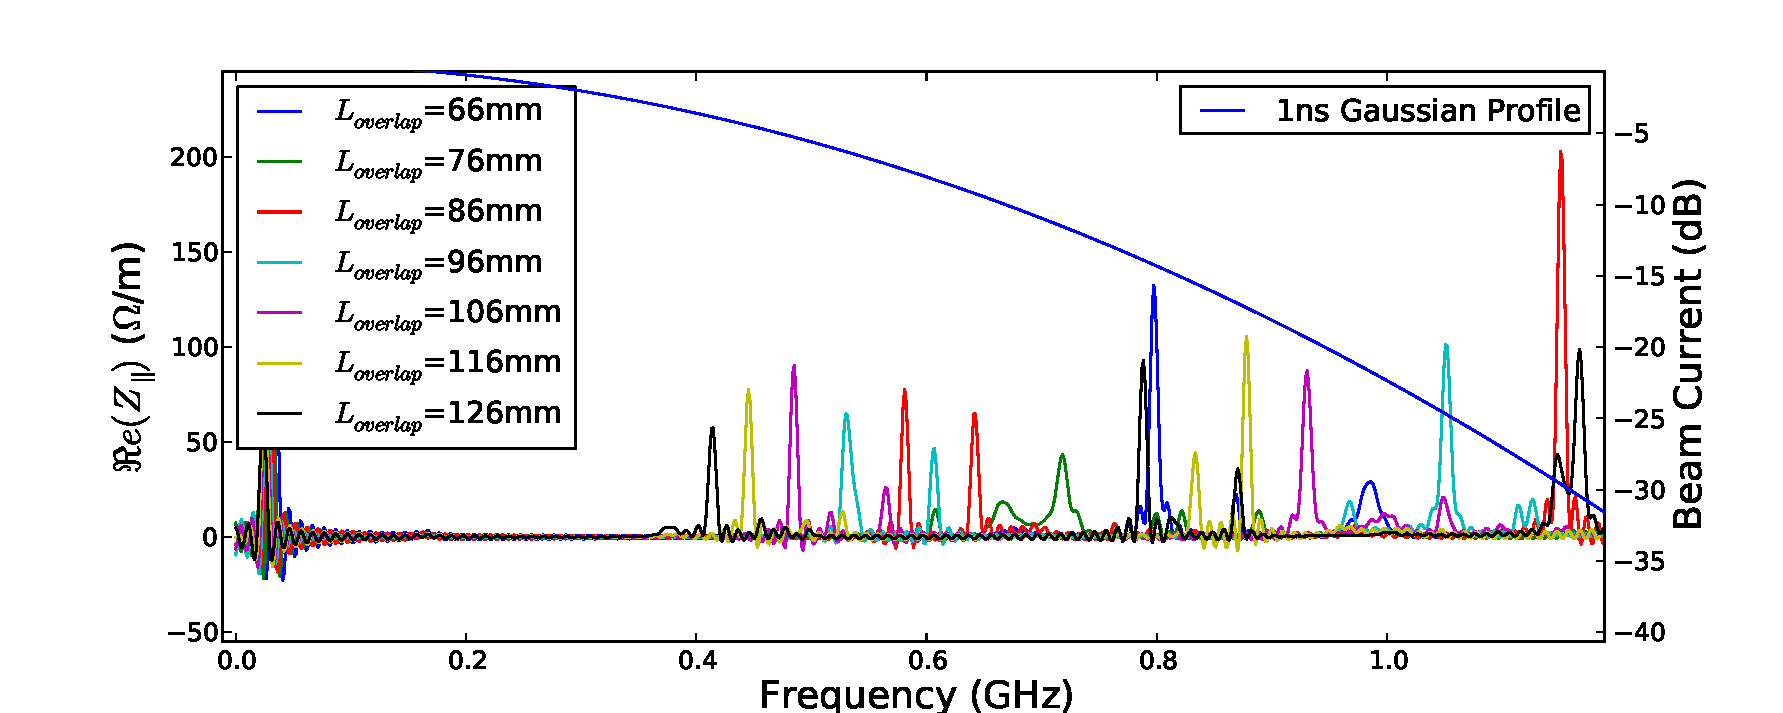
\includegraphics[width=0.8\textwidth]{TUPRI030f6.pdf}
\end{center}
\end{block}



\vfill

          }
          % ---------------------------------------------------------%
          % end the column
        \end{minipage}
      \end{beamercolorbox}
    \end{column}
    % ---------------------------------------------------------%
    % end the column
  \end{columns}

  %\tiny\hfill\textcolor{ta2gray}{Created with \LaTeX \texttt{beamerposter}  \url{http://www-i6.informatik.rwth-aachen.de/~dreuw/latexbeamerposter.php}}
%  \tiny\hfill{Created with \LaTeX \texttt{beamerposter}  \url{http://www-i6.informatik.rwth-aachen.de/~dreuw/latexbeamerposter.php} \hskip1em}
\end{frame}
\end{document}


%%%%%%%%%%%%%%%%%%%%%%%%%%%%%%%%%%%%%%%%%%%%%%%%%%%%%%%%%%%%%%%%%%%%%%%%%%%%%%%%%%%%%%%%%%%%%%%%%%%%
%%% Local Variables: 
%%% mode: latex
%%% TeX-PDF-mode: t
%%% End:
